\documentclass[t]{beamer}
\usetheme[cabin, darktitle]{UniversityOfManchester}

%% Document properties
\title{An efficient SpiNNaker implementation of the Neural~Engineering~Framework}
\author{Andrew Mundy, James Knight,\\Terry Stewart and Steve Furber}

\usepackage[binary-units]{siunitx}
\usepackage[backend=bibtex, doi=false, url=false,
            autocite=footnote, maxbibnames=3, style=authoryear]{biblatex}
\bibliography{paper}

\begin{document}
  \maketitle

  %% Constraints on SpiNNaker programs
  %% - Memory usage
  %%  - In its own right
  %%  - Time to load data
  %% - Processing time
  %%  - Dominated by synaptic weight lookup -- < 5000 synaptic events per timestep
  \begin{frame}{Simulating neural nets on SpiNNaker}
    \vfill
    \hspace*{-.15\textwidth}\includegraphics[page=2, width=1.3\textwidth]{algorithm_diagram}
    \vfill
    \pause
    Constraints on number of neurons per core:
    \begin{description}
      \item[Memory] Size of weight matrix
      \item[Compute] Number of synaptic events
    \end{description}
  \end{frame}

  \begin{frame}{Performance of the SpiNNaker architecture}
    Constraints:
    \begin{itemize}
      \item \SI{8}{\mebi\byte} limit on weight matrices.
      \item Max \num{5000} synaptic events per millisecond \parencite{Sharp2013}.
      \begin{itemize}
        \item One synaptic event is one spike for one synapse.
      \end{itemize}
    \end{itemize}

    \pause
    Overcome by:
    \begin{itemize}[<+->]
      \item Allocating fewer neurons to a core
        \begin{itemize}
          \item \textbf{but} power and number of processors limited.
        \end{itemize}
      \item Using longer simulation time-steps
        \begin{itemize}
          \item \textbf{but} sometimes hard deadlines.
        \end{itemize}
    \end{itemize}
  \end{frame}

  \begin{frame}{Bad characteristics}
    Fine for the majority of the cases, not helped by:
    \begin{itemize}
      \item Dense weight matrices
      \item High firing rates
    \end{itemize}
    \pause
    Both characteristics of models built with the Neural~Engineering~Framework~(NEF)
  \end{frame}

  %% Introduction to the NEF
  \begin{frame}{The Neural Engineering Framework (NEF)}
    \begin{itemize}
      \item Populations of neurons represent abstract values.
      \item Connections compute functions of representations.
      \item Extended by the Semantic Pointer Architecture (SPA).
    \end{itemize}
  \end{frame}

  %% - Encoding
  %% - Decoding
  %% - Forming weight matrices
  %% TODO Motivate encoding, explain decoding
  \begin{frame}[plain]{Representing scalars}
    \vfill
    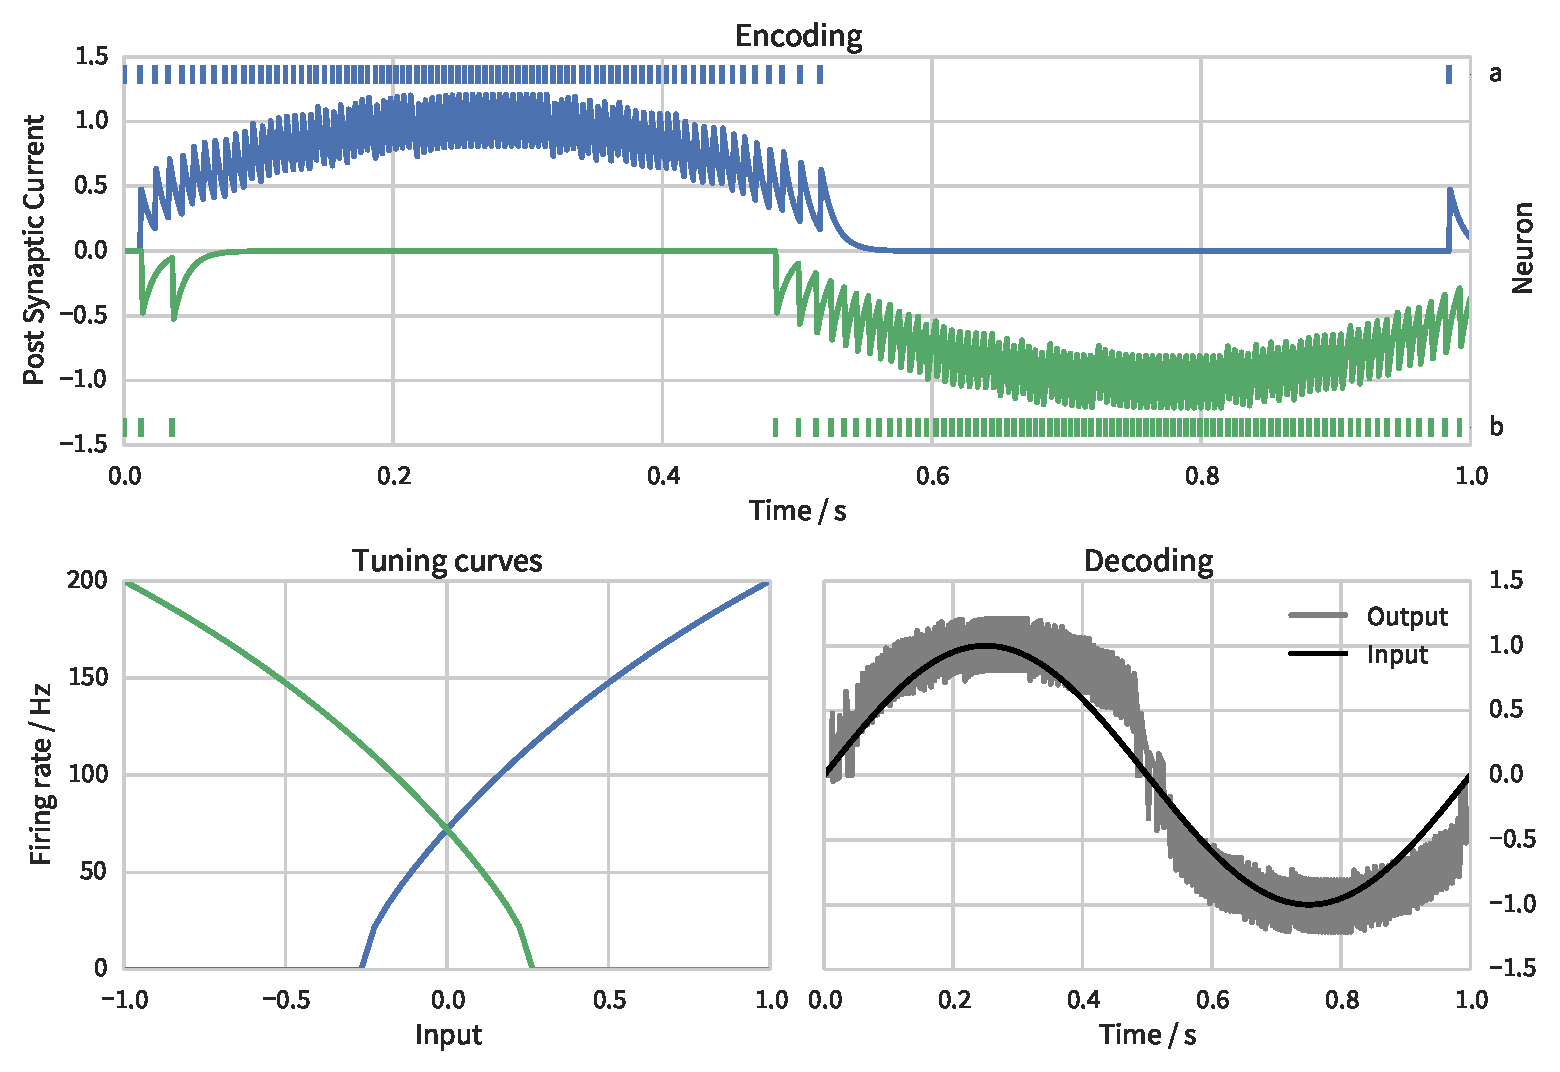
\includegraphics[width=\textwidth]{encoding_decoding}
    \vfill
  \end{frame}

  \begin{frame}[plain]{Representing vectors}
    \vfill
    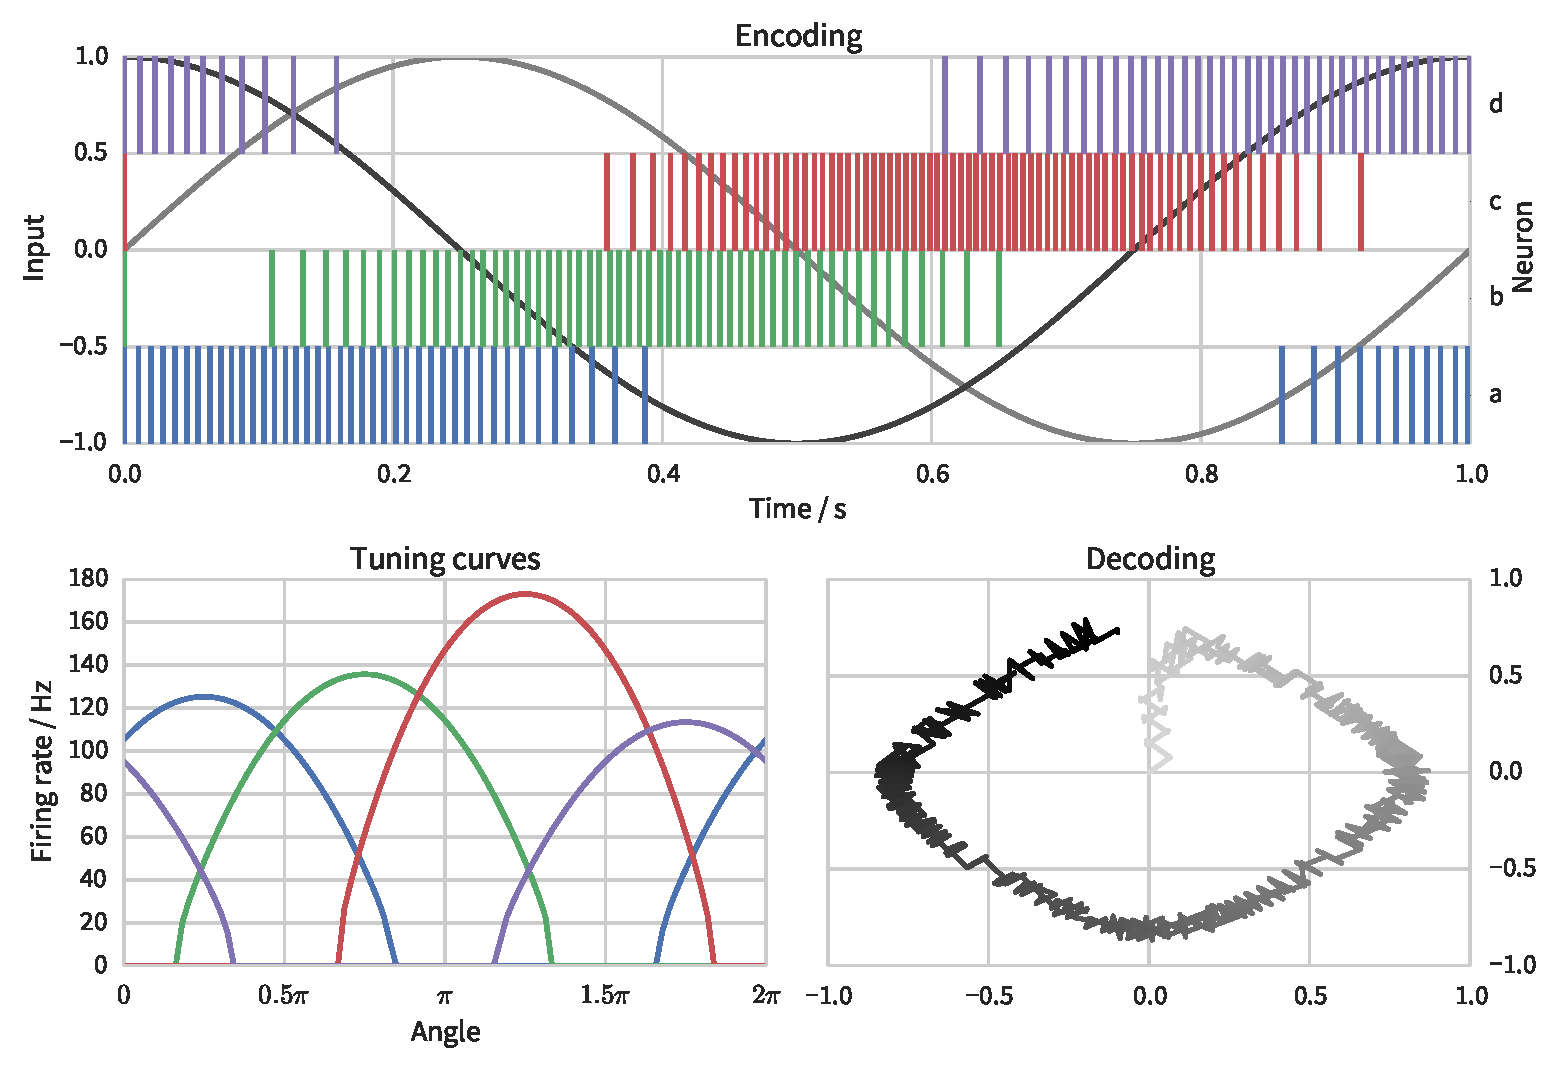
\includegraphics[width=\textwidth]{encoding_decoding2d}
    \vfill
  \end{frame}

  \begin{frame}{Combining encoding and decoding}
  \end{frame}

  %% How does the NEF meet these constraints?
  %% - Consider communication channel using Spaun-like parameters of 16-D and 70 neurons per dimension
  %%  - Memory use is insane (down to 53 neurons per core)
  %%  - Synaptic events very quickly pass the max allowed
  %% Result: using the standard approach with the NEF will lead to suboptimal use of the architecture.

  %% An alternative: value-based transmission
  %% - Note that weight matrices can be factored into encoders and decoders
  %% - Indicate how this can be used in simulation using the payloads of MC packets
  \begin{frame}{Value Transmission}
    \vfill
    \hspace*{-.15\textwidth}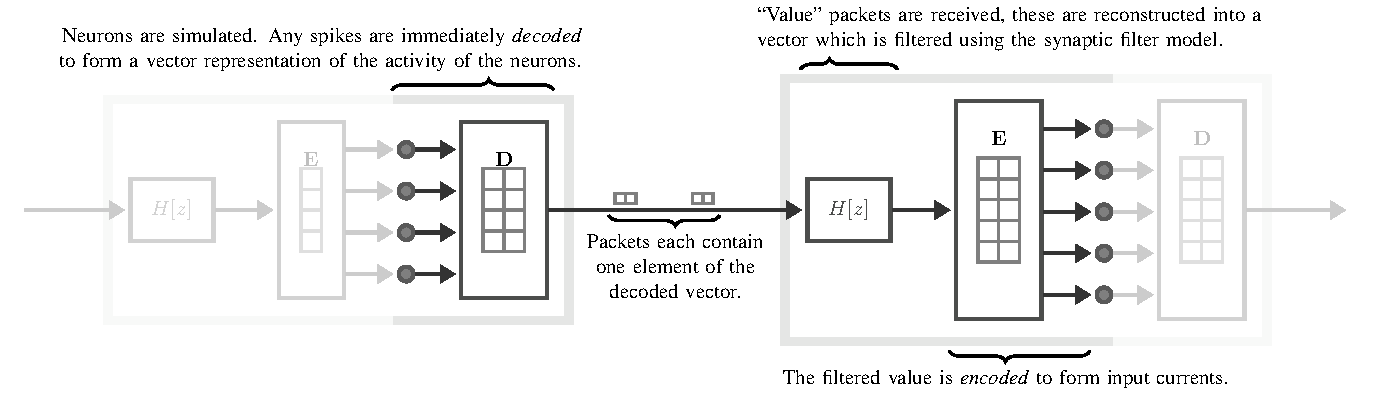
\includegraphics[page=1, width=1.3\textwidth]{algorithm_diagram}
    \vfill
    \pause
    \begin{itemize}
      \item Factored weight matrices $\ll$ full weight matrix
      \item Different compute requirements
    \end{itemize}
  \end{frame}

  %% Results
  %% - Memory usage
  %% - Processor usage

  %% Discussion (brief)

  %% Thanks!
\end{document}
